\subsection{Robot Controller Design}
\label{subsec:controllerdesign}

\begin{figure} [ht]
  \centering
  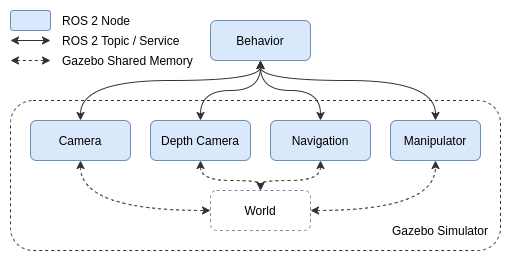
\includegraphics[width=0.45\textwidth]{images/simulation-controller.png}
  \caption{Diagram of the robot controller system in the simulation.}
  \label{fig:simulationcontroller}
\end{figure}

The robot controller used for this simulation will be developed using ROS 2.
The controller will be separated into several parts in the form of ROS 2 nodes as shown in Figure \ref{fig:simulationcontroller}.
Each existing node will be connected to each other using the ROS 2's interprocess communication system in the form of topics and services.

The main part of the robot controller is the behavior node which contains a program that regulates all robot actions based on data obtained from the sensors in the simulation.
Then the behavior node will be connected to four other nodes that represent the sensors and actuators in the robot.
Those four nodes will be attached in the scope of the Gazebo simulator as Gazebo plugins,
  so that they can be used to access and manipulate data in the simulation using the shared memory system in the Gazebo \citep{gazeboplugins}.

\begin{figure} [ht] \centering
  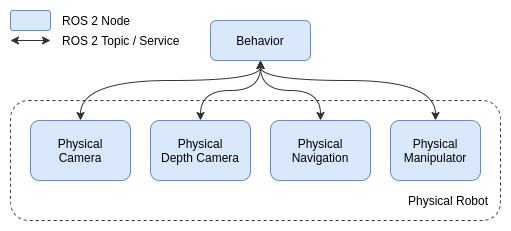
\includegraphics[width=0.45\textwidth]{images/real-robot-controller.png}
  \caption{Diagram of the real robot controller system.}
  \label{fig:realrobotcontroller}
\end{figure}

This system is designed separately so that the behavior nodes tested in the simulation environment could be used directly on the real robot.
As shown in Figure \ref{fig:realrobotcontroller},
  the transfer of controllers to the real robot can be done by changing the entire scope of the Gazebo simulator,
  which consists of the four nodes mentioned earlier,
  into nodes that process sensors and actuators on the real robot.
With this, the tests carried out in the simulation can be directly applied when tested on the real robot because there is no need to redevelop the controller that adapts to the existing system on the real robot.
